\documentclass[twoside]{book}

% Packages required by doxygen
\usepackage{fixltx2e}
\usepackage{calc}
\usepackage{doxygen}
\usepackage[export]{adjustbox} % also loads graphicx
\usepackage{graphicx}
\usepackage[utf8]{inputenc}
\usepackage{makeidx}
\usepackage{multicol}
\usepackage{multirow}
\PassOptionsToPackage{warn}{textcomp}
\usepackage{textcomp}
\usepackage[nointegrals]{wasysym}
\usepackage[table]{xcolor}

% Font selection
\usepackage[T1]{fontenc}
\usepackage[scaled=.90]{helvet}
\usepackage{courier}
\usepackage{amssymb}
\usepackage{sectsty}
\renewcommand{\familydefault}{\sfdefault}
\allsectionsfont{%
  \fontseries{bc}\selectfont%
  \color{darkgray}%
}
\renewcommand{\DoxyLabelFont}{%
  \fontseries{bc}\selectfont%
  \color{darkgray}%
}
\newcommand{\+}{\discretionary{\mbox{\scriptsize$\hookleftarrow$}}{}{}}

% Page & text layout
\usepackage{geometry}
\geometry{%
  a4paper,%
  top=2.5cm,%
  bottom=2.5cm,%
  left=2.5cm,%
  right=2.5cm%
}
\tolerance=750
\hfuzz=15pt
\hbadness=750
\setlength{\emergencystretch}{15pt}
\setlength{\parindent}{0cm}
\setlength{\parskip}{3ex plus 2ex minus 2ex}
\makeatletter
\renewcommand{\paragraph}{%
  \@startsection{paragraph}{4}{0ex}{-1.0ex}{1.0ex}{%
    \normalfont\normalsize\bfseries\SS@parafont%
  }%
}
\renewcommand{\subparagraph}{%
  \@startsection{subparagraph}{5}{0ex}{-1.0ex}{1.0ex}{%
    \normalfont\normalsize\bfseries\SS@subparafont%
  }%
}
\makeatother

% Headers & footers
\usepackage{fancyhdr}
\pagestyle{fancyplain}
\fancyhead[LE]{\fancyplain{}{\bfseries\thepage}}
\fancyhead[CE]{\fancyplain{}{}}
\fancyhead[RE]{\fancyplain{}{\bfseries\leftmark}}
\fancyhead[LO]{\fancyplain{}{\bfseries\rightmark}}
\fancyhead[CO]{\fancyplain{}{}}
\fancyhead[RO]{\fancyplain{}{\bfseries\thepage}}
\fancyfoot[LE]{\fancyplain{}{}}
\fancyfoot[CE]{\fancyplain{}{}}
\fancyfoot[RE]{\fancyplain{}{\bfseries\scriptsize Generated by Doxygen }}
\fancyfoot[LO]{\fancyplain{}{\bfseries\scriptsize Generated by Doxygen }}
\fancyfoot[CO]{\fancyplain{}{}}
\fancyfoot[RO]{\fancyplain{}{}}
\renewcommand{\footrulewidth}{0.4pt}
\renewcommand{\chaptermark}[1]{%
  \markboth{#1}{}%
}
\renewcommand{\sectionmark}[1]{%
  \markright{\thesection\ #1}%
}

% Indices & bibliography
\usepackage{natbib}
\usepackage[titles]{tocloft}
\setcounter{tocdepth}{3}
\setcounter{secnumdepth}{5}
\makeindex

% Hyperlinks (required, but should be loaded last)
\usepackage{ifpdf}
\ifpdf
  \usepackage[pdftex,pagebackref=true]{hyperref}
\else
  \usepackage[ps2pdf,pagebackref=true]{hyperref}
\fi
\hypersetup{%
  colorlinks=true,%
  linkcolor=blue,%
  citecolor=blue,%
  unicode%
}

% Custom commands
\newcommand{\clearemptydoublepage}{%
  \newpage{\pagestyle{empty}\cleardoublepage}%
}

\usepackage{caption}
\captionsetup{labelsep=space,justification=centering,font={bf},singlelinecheck=off,skip=4pt,position=top}

%===== C O N T E N T S =====

\begin{document}

% Titlepage & ToC
\hypersetup{pageanchor=false,
             bookmarksnumbered=true,
             pdfencoding=unicode
            }
\pagenumbering{alph}
\begin{titlepage}
\vspace*{7cm}
\begin{center}%
{\Large My Project }\\
\vspace*{1cm}
{\large Generated by Doxygen 1.8.13}\\
\end{center}
\end{titlepage}
\clearemptydoublepage
\pagenumbering{roman}
\tableofcontents
\clearemptydoublepage
\pagenumbering{arabic}
\hypersetup{pageanchor=true}

%--- Begin generated contents ---
\chapter{Hierarchical Index}
\section{Class Hierarchy}
This inheritance list is sorted roughly, but not completely, alphabetically\+:\begin{DoxyCompactList}
\item \contentsline{section}{Command}{\pageref{struct_command}}{}
\item \contentsline{section}{Controller}{\pageref{class_controller}}{}
\begin{DoxyCompactList}
\item \contentsline{section}{Console\+Controller}{\pageref{class_console_controller}}{}
\item \contentsline{section}{Sequence\+Controller}{\pageref{class_sequence_controller}}{}
\end{DoxyCompactList}
\item \contentsline{section}{Servo}{\pageref{class_servo}}{}
\end{DoxyCompactList}

\chapter{Class Index}
\section{Class List}
Here are the classes, structs, unions and interfaces with brief descriptions\+:\begin{DoxyCompactList}
\item\contentsline{section}{\hyperlink{struct_command}{Command} }{\pageref{struct_command}}{}
\item\contentsline{section}{\hyperlink{class_console_controller}{Console\+Controller} }{\pageref{class_console_controller}}{}
\item\contentsline{section}{\hyperlink{class_controller}{Controller} }{\pageref{class_controller}}{}
\item\contentsline{section}{\hyperlink{class_sequence_controller}{Sequence\+Controller} }{\pageref{class_sequence_controller}}{}
\item\contentsline{section}{\hyperlink{class_servo}{Servo} }{\pageref{class_servo}}{}
\end{DoxyCompactList}

\chapter{Class Documentation}
\hypertarget{struct_command}{}\section{Command Struct Reference}
\label{struct_command}\index{Command@{Command}}
\subsection*{Public Attributes}
\begin{DoxyCompactItemize}
\item 
\mbox{\Hypertarget{struct_command_a443f10e416bca15f55402458b2e03c47}\label{struct_command_a443f10e416bca15f55402458b2e03c47}} 
int {\bfseries base\+Angle}
\item 
\mbox{\Hypertarget{struct_command_ad96d921554a260d14e929d094eb1ac78}\label{struct_command_ad96d921554a260d14e929d094eb1ac78}} 
int {\bfseries upper\+Angle}
\item 
\mbox{\Hypertarget{struct_command_acd7a5e14835136f9552c11f7a384c2d4}\label{struct_command_acd7a5e14835136f9552c11f7a384c2d4}} 
int {\bfseries lower\+Angle}
\item 
\mbox{\Hypertarget{struct_command_a47af13c81ab5095a0dea24ceb7de362e}\label{struct_command_a47af13c81ab5095a0dea24ceb7de362e}} 
int {\bfseries finger\+Angle}
\end{DoxyCompactItemize}


The documentation for this struct was generated from the following file\+:\begin{DoxyCompactItemize}
\item 
controller.\+h\end{DoxyCompactItemize}

\hypertarget{class_console_controller}{}\section{Console\+Controller Class Reference}
\label{class_console_controller}\index{Console\+Controller@{Console\+Controller}}
Inheritance diagram for Console\+Controller\+:\begin{figure}[H]
\begin{center}
\leavevmode
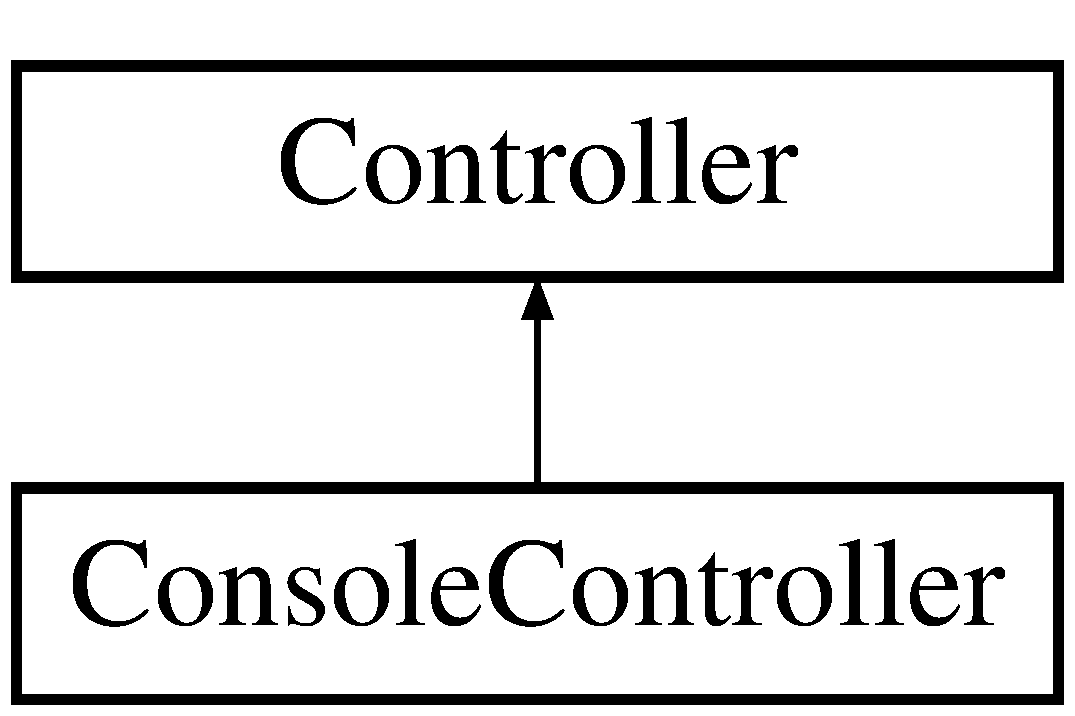
\includegraphics[height=2.000000cm]{class_console_controller}
\end{center}
\end{figure}
\subsection*{Public Member Functions}
\begin{DoxyCompactItemize}
\item 
\mbox{\Hypertarget{class_console_controller_a43ba6c4a33ed626692eaea2d534fe370}\label{class_console_controller_a43ba6c4a33ed626692eaea2d534fe370}} 
\hyperlink{struct_command}{Command} {\bfseries get\+Command} ()
\end{DoxyCompactItemize}


The documentation for this class was generated from the following files\+:\begin{DoxyCompactItemize}
\item 
controller.\+h\item 
controller.\+cpp\end{DoxyCompactItemize}

\hypertarget{class_controller}{}\section{Controller Class Reference}
\label{class_controller}\index{Controller@{Controller}}
Inheritance diagram for Controller\+:\begin{figure}[H]
\begin{center}
\leavevmode
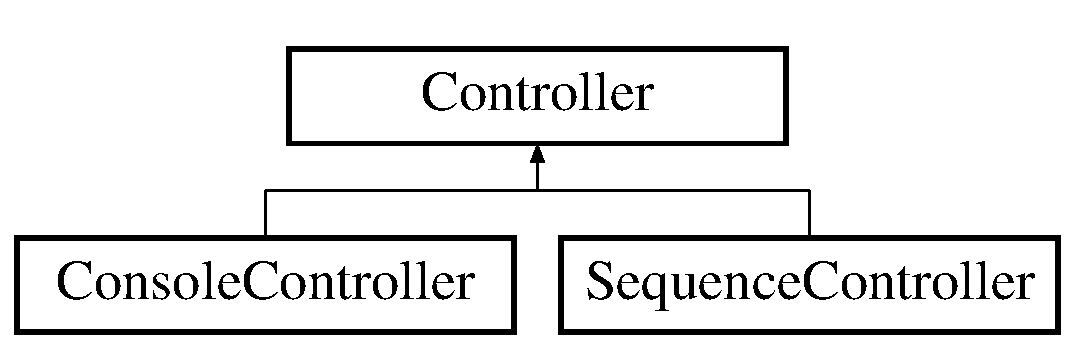
\includegraphics[height=2.000000cm]{class_controller}
\end{center}
\end{figure}
\subsection*{Public Member Functions}
\begin{DoxyCompactItemize}
\item 
\mbox{\Hypertarget{class_controller_a84257cfce42e5565c29f11ef7e86d10a}\label{class_controller_a84257cfce42e5565c29f11ef7e86d10a}} 
virtual \hyperlink{struct_command}{Command} {\bfseries get\+Command} ()=0
\end{DoxyCompactItemize}


The documentation for this class was generated from the following file\+:\begin{DoxyCompactItemize}
\item 
controller.\+h\end{DoxyCompactItemize}

\hypertarget{class_sequence_controller}{}\section{Sequence\+Controller Class Reference}
\label{class_sequence_controller}\index{Sequence\+Controller@{Sequence\+Controller}}
Inheritance diagram for Sequence\+Controller\+:\begin{figure}[H]
\begin{center}
\leavevmode
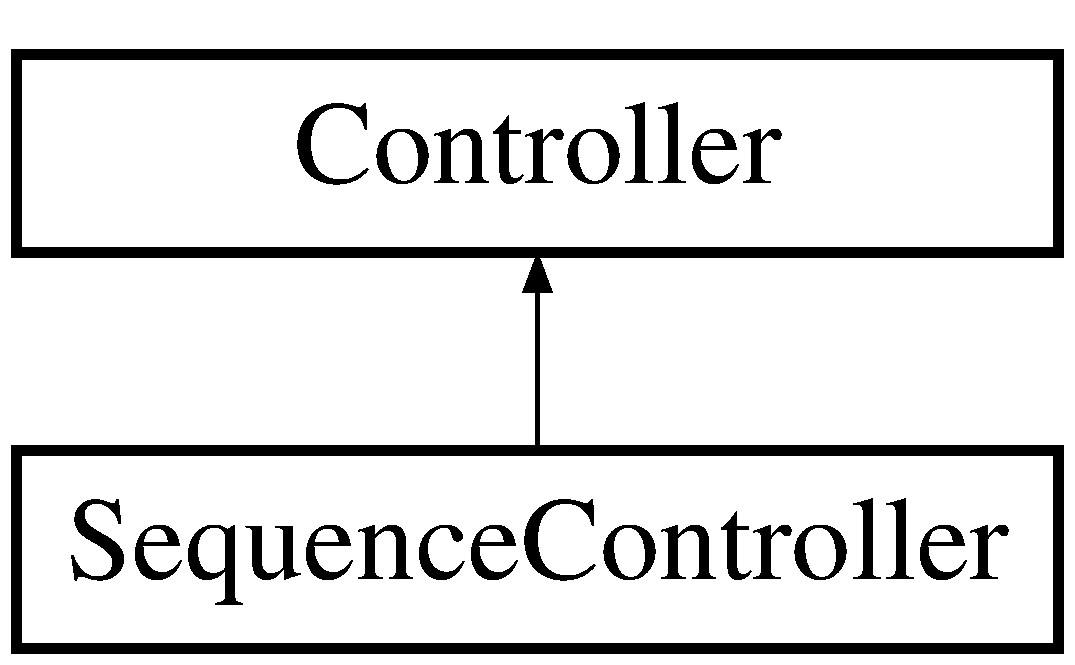
\includegraphics[height=2.000000cm]{class_sequence_controller}
\end{center}
\end{figure}
\subsection*{Public Member Functions}
\begin{DoxyCompactItemize}
\item 
\mbox{\Hypertarget{class_sequence_controller_a45bc2951b1783dd32abfe4e79554473f}\label{class_sequence_controller_a45bc2951b1783dd32abfe4e79554473f}} 
\hyperlink{struct_command}{Command} {\bfseries get\+Command} ()
\end{DoxyCompactItemize}


The documentation for this class was generated from the following files\+:\begin{DoxyCompactItemize}
\item 
controller.\+h\item 
controller.\+cpp\end{DoxyCompactItemize}

\hypertarget{class_servo}{}\section{Servo Class Reference}
\label{class_servo}\index{Servo@{Servo}}
\subsection*{Public Member Functions}
\begin{DoxyCompactItemize}
\item 
\mbox{\Hypertarget{class_servo_abfe85df93271b5d0e54b9cee6c50abc6}\label{class_servo_abfe85df93271b5d0e54b9cee6c50abc6}} 
{\bfseries Servo} (char $\ast$a\+Name, int pin\+Index, int a\+Min, int a\+Max, int initial, int offset, bool invert)
\item 
\mbox{\Hypertarget{class_servo_acc048b630aca0383409074e16ee521d4}\label{class_servo_acc048b630aca0383409074e16ee521d4}} 
{\bfseries rotate\+To} (int angle)
\end{DoxyCompactItemize}


The documentation for this class was generated from the following files\+:\begin{DoxyCompactItemize}
\item 
servo.\+h\item 
servo.\+cpp\end{DoxyCompactItemize}

%--- End generated contents ---

% Index
\backmatter
\newpage
\phantomsection
\clearemptydoublepage
\addcontentsline{toc}{chapter}{Index}
\printindex

\end{document}
